\tikzset{weights/.pic={
         code={
            %\tikzset{scale=5/10}
            \newcommand{\x}{0}
            \newcommand{\xb}{\x+0.3}
            \newcommand{\xc}{\x+0.6}
            \newcommand{\hf}{1.25}  % height front
            \newcommand{\hb}{1}  % height back
            \newcommand{\w}{1.2}  % width
            \newcommand{\y}{3.25}
            \filldraw[fill=white] (\xc, \y) -- (\xc, \y+\hb) -- (\xc+\w, \y+\hf) -- (\xc+\w,\y-0.25) -- (\xc, \y);
            \filldraw[fill=white] (\xb, \y) -- (\xb, \y+\hb) -- (\xb+\w, \y+\hf) -- (\xb+\w, \y-0.25) -- (\xb, \y);
            \filldraw[fill=white] (\x, \y) -- (\x, \y+\hb) -- (\x+\w, \y+\hf) -- (\x+\w,\y-0.25) -- (\x, \y);
            \node at (\x + 0.66, \y + 0.5) {$\mathbf{W}, b$};
  }}
}

\begin{figure}[t]
    \begin{center}
    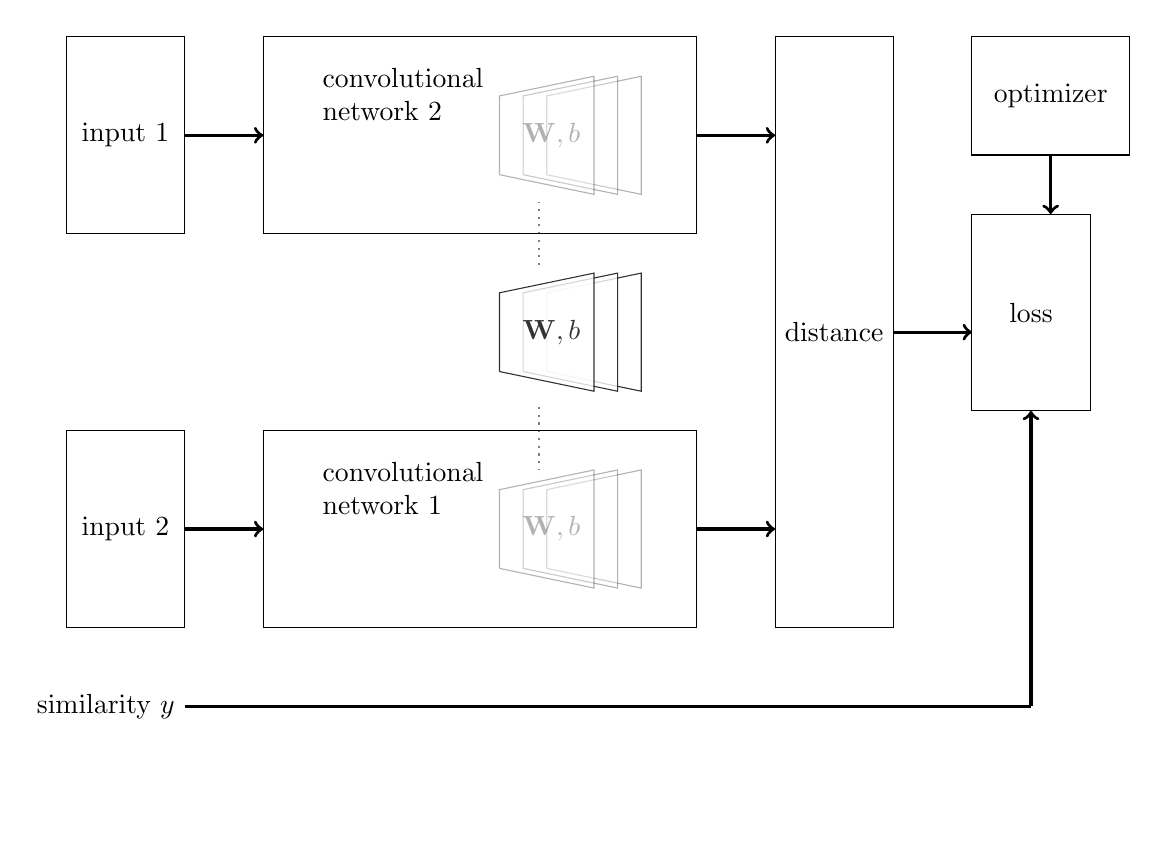
\begin{tikzpicture}
        %conv nets
        \draw (2,5) rectangle (7.5,7.5) node[label={[shift={(-33ex,-1ex)}, align = left]south east:convolutional \\network 2}] {};
        \draw (2,0) rectangle (7.5,2.5) node[label={[shift={(-33ex,-1ex)}, align = left]south east:convolutional \\ network 1}] {};
        
        % distance
        \draw[->,very thick] (7.5,1.25) -- (8.5,1.25);
        \draw[->,very thick] (7.5,6.25) -- (8.5,6.25);
        \draw (8.5,0) rectangle (10,7.5) node[pos=.5] {distance};

        % optimizer
        \draw[->,very thick] (12, 6) -- (12, 5.25);
        \draw (11, 6) rectangle (13, 7.5) node[pos=.5] {optimizer};

        % loss
        \draw[->,very thick] (10,3.75) -- (11,3.75);
        \draw (11, 2.75) rectangle (12.5, 5.25) node[pos=.5] {loss};
        
        % inputs
        \draw[->,very thick] (1,1.25) -- (2,1.25);
        \draw[->,very thick] (1,6.25) -- (2,6.25);
        \draw (-0.5,5) rectangle (1,7.5) node[pos=.5] {input 1};
        \draw (-0.5,0) rectangle (1,2.5) node[pos=.5] {input 2};

        % similarity label
        \draw[->,very thick] (11.75,-1) -- (11.75,2.75);
        \draw[-,very thick] (1,-1) -- (11.75,-1);
        \node at (0, -1) {similarity $y$};

        % weights
        \path (5,0) pic {weights}[opacity=0.8];
        \path (5,2.5) pic {weights}[opacity=0.3];
        \path (5,-2.5) pic {weights}[opacity=0.3];

        \draw[-, dotted, thick, opacity=0.5] (5.5,4.6) -- (5.5,5.4);
        \draw[-, dotted, thick, opacity=0.5] (5.5,2.8) -- (5.5, 2);
        

    \end{tikzpicture}
    \end{center}
    \caption[Structure of a siamese neural network]{\textbf{Structure of a siamese neural network.} The two convolutional networks share the weights $\mathbf{W}$ and biases $b$. The distance between the output vectors of the two networks is fed into the the contrastive loss function. The contrastive loss penalizes small or large distances, depending on the similarity label $y$.}
    \label{fig:Siamese}
\end{figure}